\subsection{Source-Line Hints on New Receipts}
\label{sec:eval:receipt_followup}

In the first 60-receipt test, base and error-report prompts keep all input
graphs unchanged. Filtering lowers F1 from 79.44\% to 79.15\%.
It rejects an address because its spaces differ from the source.
Of 49 reference differences, 27 involve case, spaces, punctuation, or amount
format (Appendix~\ref{sec:eval:external_receipts}). We use these findings to
add field meanings, source-line hints, and a shared whitespace rule.

We set the index design on 20 new receipts, then fix it before testing 60
further receipts (Section~\ref{sec:framework:field_evidence}).
The first 60, development 20, and new test 60 receipts have different IDs
and different text after whitespace cleanup. Sampling uses seed 20260923.
Test labels are downloaded after all predictions are saved.
Every method receives the same field meanings, numbered source lines,
input graph, and instructions. Simple uses them directly.
Evidence Index adds field-line hints. SHACL adds rule-check context.
All three use the same whitespace rule in the filter.

Development F1 is 80.00\% for the input, 82.50\% for Simple,
85.00\% for Evidence Index, and 80.00\% for SHACL.
We keep one index design and all three methods for the test.
The main comparison is Evidence Index minus Simple in mean document F1.
The code and scoring rules are fixed before testing.

\begin{table*}[t]
\centering
\caption{Repair on 60 new receipts. Methods share field meanings, source lines, and the same whitespace check. Exact match uses the labelled fields.}
\label{tab:receipt_followup}
\small
\begin{tabular}{lrrrr}
\toprule
Method & Triple F1 & Exact graph & Normalized F1 & Facts kept \\
\midrule
Extracted input & 0.7833 & 0.3500 & 0.7958 & 1.0000 \\
Simple, raw & 0.7875 & 0.2833 & 0.8083 & 0.9250 \\
Simple, gate & 0.7875 & 0.2833 & 0.8083 & 0.9250 \\
Evidence Index, raw & 0.8333 & 0.4000 & 0.8625 & 0.9306 \\
Evidence Index, gate & 0.8351 & 0.4000 & 0.8643 & 0.9306 \\
SHACL context, raw & 0.7833 & 0.2833 & 0.8042 & 0.9347 \\
SHACL context, gate & 0.7833 & 0.2833 & 0.8042 & 0.9347 \\
\bottomrule
\end{tabular}
\end{table*}

On the new test, input F1 is 78.33\%. Simple, Evidence Index, and SHACL
reach 78.75\%, 83.51\%, and 78.33\% after filtering.
Simple gains $0.42$ points over the input (95\% CI: $[-4.17,5.00]$).
Evidence Index leads Simple by $4.76$ points
(95\% CI: $[2.50,7.26]$; paired randomization $p=0.0004$).
Exact match is 28.33\%, 40.00\%, and 28.33\% for the three methods.

The input has 52 fields that differ from the reference.
Simple recovers 16 of them and loses 15 exact input matches.
Evidence Index recovers 26 and loses 14. SHACL recovers 13 and loses 13.
The index fixes 11 punctuation differences and 6 text-boundary differences.
Among its 14 lost exact matches, 10 keep the same numeric amount and change
the display format.

A numeric check removes currency prefixes and thousands separators from
the total field. It gives 58/60 correct amounts for the input,
59/60 for Simple, 59/60 for Evidence Index, and 58/60 for SHACL.
After case and whitespace cleanup, F1 is 86.43\% for Evidence Index
and 80.83\% for Simple. The index improves both exact and cleaned-text scores.

The filter rejects 1 candidate. It differs from the reference and joins
address parts into text absent from the source. The count of rejected
reference matches is 0. Filtering raises indexed F1 by 0.18 points.
The other two methods keep the same F1.

Simple, Evidence Index, and SHACL change 31, 39, and 28 input graphs.
Their mean repair request times are 7.91, 7.88, and 8.11 seconds.
Mean input lengths are 1784, 2153, and 3404 tokens.
The 240 requests produce 60 extraction and 180 repair outputs.
Request times include pacing and retries. Each raw/gated score pair uses
one response.

\begin{figure}[t]
\centering
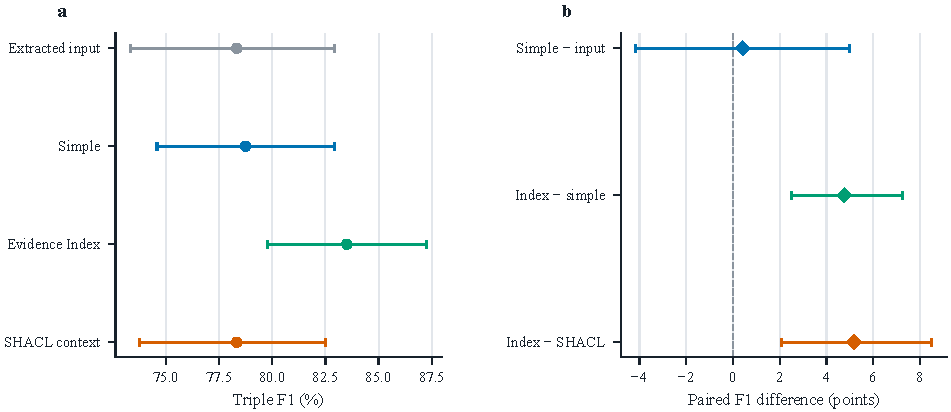
\includegraphics[width=0.98\textwidth]{figure/experiments/receipt_followup.pdf}
\caption{New receipt test. Left: mean F1 with 95\% document-bootstrap CIs. Right: paired F1 changes. All methods share field meanings and source lines.}
\label{fig:receipt_followup}
\end{figure}
